\documentclass[pdftex,12pt,a4paper]{article}
\usepackage[pdftex]{graphicx}
\usepackage{xcolor}
\usepackage{marginnote}
\usepackage{enumitem}
\usepackage[hidelinks]{hyperref}
\usepackage[bottom=1.5cm, outer=5cm, inner=2cm, heightrounded,
marginparwidth=4cm, marginparsep=0.5cm]{geometry}

\begin{document}
    % Custom title page
    \begin{titlepage}
        \begin{center}
            
\includegraphics[width=5cm]{figures/kulogo}\\[1cm]
            {\Large \bfseries
                Spring 2014\\
                Computer Networks\\
                CMPE323\\[1cm]
            }
            {\large \bfseries
                \noindent Laboratory Experiment No. 10: Miscellaneous
                Protocols\\[1cm]
            }
        \end{center}

        \noindent \textbf{Aims and Objectives:}
            \begin{itemize}[leftmargin=4cm]
                \item Introducing Dynamic Host Configuration Protocol (DHCP),
                \item and Domain Name System (DNS) protocols.
            \end{itemize}
            \vspace{0.5cm}

        \noindent \textbf{Materials Required:}
            \begin{itemize}[leftmargin=4cm]
                \item IP routers,
                \item PCs with Ethernet adapters,
                \item and straight-through/crossover/rollover cables.
            \end{itemize}
            \vspace{0.5cm}

        \noindent \textbf{Change Log:}
            \begin{itemize}[leftmargin=4cm]
                \item 20-5-2014: original document -- mkhonji.
                \item 21-5-2014: changed \texttt{r1.example.com} to
                    \texttt{pc1.example.com}, and removed the sentence
                    ``\emph{for the name servers instead}'' -- mkhonji.
                \item 23-5-2014: changed the command \texttt{ip dns enable} to
                    \texttt{ip dns server} -- mkhonji.
            \end{itemize}
    \end{titlepage}
    \newpage

    % Lab script content
    \section{Introduction}
        This lab covers a few common protocols, namely:
        \begin{itemize}
            \item Dynamic Host Configuration Protocol (DHCP) --- a protocol
                that can dynamically inform the clients which parameters they
                should set. Such parameters could be: client's IP address and
                its subnet mask, client's default gateway address, the DNS
                server to use. 
                
                The full list of such parameters can be found in the page \
                \url{https://www.iana.org/assignments/bootp-dhcp-parameters/bootp-dhcp-parameters.xhtml}.
                As you see, the list is quite extensive. However, we will only
                use the most commonly used options.
            \item Domain Name System (DNS) --- a protocol that allows using
                \emph{names} (such as Google.com) instead of numbers (such as
                IPv4, IPv6, phone numbers, port numbers, public keys, or even
                other names) throughout what is called Resource Records
                (RR).  For example, instead of memorizing the IP address of
                Google servers (which are many), you memorize the name
                \texttt{google.com}. 
                
                The DNS protocol is fairly extensive as far as it relates to
                the RRs which can be found in the page \
                \url{https://www.iana.org/assignments/dns-parameters/dns-parameters.xhtml}.
                However, in this lab we will cover the most widely-used DNS RR,
                namely the \texttt{A} RR which resolves names into IPv4
                numbers. E.g. \texttt{ping google.com} would work by
                transparently resolving \texttt{google.com} into some IPv4
                address such as \texttt{173.194.35.32}.
        \end{itemize}


        \subsection{DHCP}
            Figure \ref{fig:dhcpinteraction} depicts the interaction example
            between a DHCP client and  two DHCP servers, using the DHCP message
            types: \texttt{DHCPDISCOVER, DHCPOFFER, DHCPREQUEST, DHCPACK,
            DHCPRELEASE}.  

            \begin{figure}[!htb]
                \centering
            \begin{verbatim}
                Server          Client          Server
            (not selected)                    (selected)

                  v               v               v
                  |               |               |
                  |     Begins initialization     |
                  |               |               |
                  | _____________/|\____________  |
                  |/DHCPDISCOVER | DHCPDISCOVER  \|
                  |               |               |
              Determines          |          Determines
             configuration        |         configuration
                  |               |               |
                  |\             |  ____________/ |
                  | \________    | /DHCPOFFER     |
                  | DHCPOFFER\   |/               |
                  |           \  |                |
                  |       Collects replies        |
                  |             \|                |
                  |     Selects configuration     |
                  |               |               |
                  | _____________/|\____________  |
                  |/ DHCPREQUEST  |  DHCPREQUEST\ |
                  |               |               |
                  |               |     Commits configuration
                  |               |               |
                  |               | _____________/|
                  |               |/ DHCPACK      |
                  |               |               |
                  |    Initialization complete    |
                  |               |               |
                  .               .               .
                  .               .               .
                  |               |               |
                  |      Graceful shutdown        |
                  |               |               |
                  |               |\ ____________ |
                  |               | DHCPRELEASE  \|
                  |               |               |
                  |               |        Discards lease
                  |               |               |
                  v               v               v\end{verbatim}
                \caption{DHCP client-server interaction timeline --- Source RFC2131.}
                \label{fig:dhcpinteraction}
            \end{figure}

            All DHCP messages are formated as depicted in Figure
            \ref{fig:dhcp}. What makes different DHCP messages have different
            types is the inclusion of of the option \texttt{53} which indicates
            the type of the message.
        

            \begin{figure}[!htb]
                \centering
            \begin{verbatim}0                   1                   2                   3
0 1 2 3 4 5 6 7 8 9 0 1 2 3 4 5 6 7 8 9 0 1 2 3 4 5 6 7 8 9 0 1
+-+-+-+-+-+-+-+-+-+-+-+-+-+-+-+-+-+-+-+-+-+-+-+-+-+-+-+-+-+-+-+-+
|     op (1)    |   htype (1)   |   hlen (1)    |   hops (1)    |
+---------------+---------------+---------------+---------------+
|                            xid (4)                            |
+-------------------------------+-------------------------------+
|           secs (2)            |           flags (2)           |
+-------------------------------+-------------------------------+
|                          ciaddr  (4)                          |
+---------------------------------------------------------------+
|                          yiaddr  (4)                          |
+---------------------------------------------------------------+
|                          siaddr  (4)                          |
+---------------------------------------------------------------+
|                          giaddr  (4)                          |
+---------------------------------------------------------------+
|                                                               |
|                          chaddr  (16)                         |
|                                                               |
|                                                               |
+---------------------------------------------------------------+
|                                                               |
|                          sname   (64)                         |
+---------------------------------------------------------------+
|                                                               |
|                          file    (128)                        |
+---------------------------------------------------------------+
|                                                               |
|                          options (variable)                   |
+---------------------------------------------------------------+\end{verbatim}
                \caption{DHCP message format --- Source RFC2131.}
                \label{fig:dhcp}
            \end{figure}

            \subsubsection{DHCP header fields}
                \begin{itemize}
                    \item \texttt{op} --- operation code, 0 for request,
                        1 for response.
                    \item \texttt{htype} --- hardware type, 1 for Ethernet.
                    \item \texttt{hlen} --- hardware address length, 6 for
                        Ethernet as MAC addresses are made of 6 octets.
                    \item \texttt{hops} --- hops between the client and
                        the DHCP server. Usually 0 unless some DHCP relay
                        exists in the path by which the hop count increases.
                    \item \texttt{xid} --- transaction ID to set
                        different request/response messages apart from each
                        other.
                    \item \texttt{secs} --- seconds elapsed since the first request.
                    \item \texttt{flags} --- as of RFC 2131 only one flag bit
                        is defined, which is the \texttt{BROADCAST} flag. If
                        the flag is set (left-most bit) then DHCP servers would
                        respond to requests by broadcasts (a case when clients
                        cannot handle unicast IP packets when not having an IP
                        configured).
                    \item \texttt{ciaddr} --- the current IP address of the
                        client in case the client has one.
                    \item \texttt{yiaddr} --- the IP address given to the
                        client by the server.
                    \item \texttt{siaddr} --- next server's IP address. The
                        server is basically informing the client which server
                        should it communicate to if the client wishes to renew
                        its IP address. Usually set to the IP address of the
                        DHCP server itself.
                    \item \texttt{giaddr} --- the IP address of the DHCP relay
                        agent in case there is one between the client and the
                        DHCP server. DHCP relay agents are used to allow DHCP
                        clients messages reach DHCP servers that are located in
                        different networks. For example, a single DHCP server
                        can exist in servers network and handle requests from
                        all clients across different networks (thanks to DHCP
                        relays).
                    \item \texttt{chaddr} --- the hardware address of the
                        client (MAC address in case of Ethernet).
                    \item \texttt{sname} --- server's host name (optional).
                    \item \texttt{file} --- path to a file name that contains
                        an image that can in turn allow the DHCP clients to
                        boot.
                    \item \texttt{options} --- a list of optional fields.
                \end{itemize}

            \subsubsection{DHCP common options}
                The options are basically Type-Length-Value (TLV) elements that
                are defined by: type of the element, length of the value, and
                the value itself.

                \begin{itemize}
                    \item DHCP  message type:

                        \begin{figure}[!h]
                            \centering
                        \begin{verbatim}    Code   Len  Type
   +-----+-----+-----+
   |  53 |  1  | 1-9 |
   +-----+-----+-----+\end{verbatim}
                        \end{figure}

                        \begin{enumerate}
                            \item \texttt{DHCPDISCOVER}.
                            \item \texttt{DHCPOFFER}.
                            \item \texttt{DHCPREQUEST}.
                            \item \texttt{DHCPDECLINE}.
                            \item \texttt{DHCPACK}.
                            \item \texttt{DHCPNAK}.
                            \item \texttt{DHCPRELASE}.
                            \item \texttt{DHCPINFORM}.
                        \end{enumerate}

                    \item Subnet mask:

                        \begin{figure}[!h]
                            \centering
                        \begin{verbatim}    Code   Len        Subnet Mask
   +-----+-----+-----+-----+-----+-----+
   |  1  |  4  |  m1 |  m2 |  m3 |  m4 |
   +-----+-----+-----+-----+-----+-----+\end{verbatim}
                        \end{figure}

                    \item DNS server:

                        \begin{figure}[!h]
                            \centering
                        \begin{verbatim}    Code   Len         Address 1               Address 2
   +-----+-----+-----+-----+-----+-----+-----+-----+--
   |  6  |  n  |  a1 |  a2 |  a3 |  a4 |  a1 |  a2 |  ...
   +-----+-----+-----+-----+-----+-----+-----+-----+--\end{verbatim}
                        \end{figure}

                 \end{itemize}

        \subsection{DNS}
            Figure \ref{fig:dnsnamespace} depicts the hierarchical architecture
            of DNS which allows different DNS servers to be responsible for
            different subsets of the name space. 

            \begin{figure}[tbh]
                \centering
                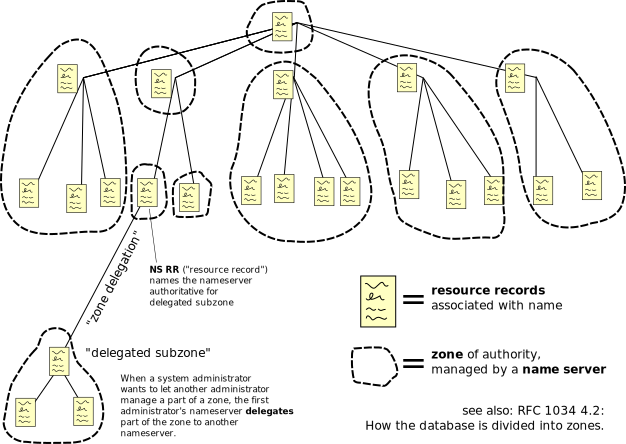
\includegraphics[width=0.9\textwidth]{figures/Domain_name_space}
                \caption{DNS name space --- Source:
                \url{http://en.wikipedia.org/wiki/File:Domain_name_space.svg}.}
                \label{fig:dnsnamespace}
            \end{figure}

            To explain how DNS works, let's take the following example:
            ``\texttt{www.google.com.}''.

            All DNS resolvers attempt to resolve the \texttt{www.google.com.}.
            All of the resolver types return an answer (i.e. resolve the name)
            if the name is known previously (i.e. cached). However, the
            resolvers behave differently if the name is not known (i.e. not
            cached):
            \begin{itemize}
                \item Non-recursive resolvers --- such resolvers will attempt to
                    resolve the name \texttt{www.google.com.} in case they know the
                    answer (e.g. cached). However, if they don't know the
                    answer, they will return the address of \emph{another} DNS
                    server that is expected to know the answer.

                    For example, if some non-recursive DNS server is queried for
                    \texttt{www.google.com.} and it does know the server that
                    knows about names below \texttt{google.com.} but does not
                    know about the full \texttt{www.google.com.} name, then it
                    will respond with the address of the authoritative DNS
                    server that is responsible for names under the name
                    \texttt{google.com}.

                    If an implementation contacts a non-recursive DNS resolver
                    to resolve names such as \texttt{www.google.com.}, the
                    implementation will have to perform the recursion by itself
                    (by recursively following the suggested authoritative name
                    servers).

                \item Recursive resolvers --- when such resolver is
                    queried, it will attempt to resolve the queried name. If
                    the name exists in its cache, it will return it
                    immediately. However, if the queried name does not exist in
                    its cache, it will contact other DNS servers and (if
                    needed) follow recursively with other DNS servers until it
                    knows the answer to the original query.

                    Implementations that query recursive DNS servers, they are
                    not required to perform the recursion by themselves as the
                    recursive DNS server will perform it until the answer to
                    the original query is found.
            \end{itemize}


            All DNS messages are formatted as depicted in Figure \ref{fig:gen}.
            \begin{figure}[!htb]
                \centering
            \begin{verbatim}    +---------------------+
    |        Header       |
    +---------------------+
    |       Question      | the question for the name server
    +---------------------+
    |        Answer       | RRs answering the question
    +---------------------+
    |      Authority      | RRs pointing toward an authority
    +---------------------+
    |      Additional     | RRs holding additional information
    +---------------------+\end{verbatim}
                \caption{DNS message format --- Source RFC1035.}
                \label{fig:gen}
            \end{figure}

            The DNS header is formatted as depicted in Figure \ref{fig:hdr},
            where \texttt{ID} is the transaction ID, \texttt{QR} is a bit that
            is 0 when the message is a DNS query and 1 when it's a response,
            \texttt{Opcode} specifies the query type (e.g. 0 for standard
            query, 1 for inverse query), \texttt{AA} is a bit that is 1 if the
            response is from an authoritative DNS server and 0 if otherwise,
            \texttt{TC} is a bit that indicates if the message was truncated
            along the path, \texttt{RD} is a bit that indicates if recursion
            DNS resolution is preferred, \texttt{RA} is a bit that indicates if
            recursive DNS resolution is available, \texttt{Z} is a set of bits
            that are reserved as of RFC1035 (some of its bits are used by now),
            \texttt{RCODE} is the response code (e.g. 0 for no error, 1 for
            request format error, 2 for internal server error, etc),
            \texttt{QDCOUNT} is the total number of queries, \texttt{ANCOUNT}
            is the total number of answers, \texttt{NSCOUNT} is the total
            number of authoritative DNS server answers, \texttt{ARCOUNT} is the
            total number of additional RRs.
            \begin{figure}[!htb]
                \centering
            \begin{verbatim}                                    1  1  1  1  1  1
      0  1  2  3  4  5  6  7  8  9  0  1  2  3  4  5
    +--+--+--+--+--+--+--+--+--+--+--+--+--+--+--+--+
    |                      ID                       |
    +--+--+--+--+--+--+--+--+--+--+--+--+--+--+--+--+
    |QR|   Opcode  |AA|TC|RD|RA|   Z    |   RCODE   |
    +--+--+--+--+--+--+--+--+--+--+--+--+--+--+--+--+
    |                    QDCOUNT                    |
    +--+--+--+--+--+--+--+--+--+--+--+--+--+--+--+--+
    |                    ANCOUNT                    |
    +--+--+--+--+--+--+--+--+--+--+--+--+--+--+--+--+
    |                    NSCOUNT                    |
    +--+--+--+--+--+--+--+--+--+--+--+--+--+--+--+--+
    |                    ARCOUNT                    |
    +--+--+--+--+--+--+--+--+--+--+--+--+--+--+--+--+\end{verbatim}
                \caption{DNS header format --- Source RFC1035.}
                \label{fig:hdr}
            \end{figure}

            The \texttt{Question} format is depicted in Figure
            \ref{fig:question}, where \texttt{QNAME} is the name to be
            resolved, \texttt{QTYPE} is the queried RR type (e.g. A, MX, TXT,
            etc), and \texttt{QCLASS} is the queried RR class (e.g. 1 for Internet
            (aka IN)).
            \begin{figure}[!htb]
                \centering
            \begin{verbatim}                                    1  1  1  1  1  1
      0  1  2  3  4  5  6  7  8  9  0  1  2  3  4  5
    +--+--+--+--+--+--+--+--+--+--+--+--+--+--+--+--+
    |                                               |
    /                     QNAME                     /
    /                                               /
    +--+--+--+--+--+--+--+--+--+--+--+--+--+--+--+--+
    |                     QTYPE                     |
    +--+--+--+--+--+--+--+--+--+--+--+--+--+--+--+--+
    |                     QCLASS                    |
    +--+--+--+--+--+--+--+--+--+--+--+--+--+--+--+--+\end{verbatim}
                \caption{DNS question format --- Source RFC1035.}
                \label{fig:question}
            \end{figure}


            All query answer RRs, authoritative RRs and additional RRs share
            the same format as depicted in Figure \ref{fig:rr}, where
            \texttt{NAME} is the domain name, \texttt{TYPE} is the RR type
            (e.g. A, MX, TXT, etc), \texttt{CLASS} is the data class (e.g. 1
            for IN), \texttt{TTL} is the total number of seconds the answer is
            advised to be cached, \texttt{RDLENGTH} is the data length in
            octets, \texttt{RDATA} is the RR's data (e.g. IPv4 address, another
            name, etc).
            \begin{figure}[!htb]
                \centering
            \begin{verbatim}                                    1  1  1  1  1  1
      0  1  2  3  4  5  6  7  8  9  0  1  2  3  4  5
    +--+--+--+--+--+--+--+--+--+--+--+--+--+--+--+--+
    |                                               |
    /                                               /
    /                      NAME                     /
    |                                               |
    +--+--+--+--+--+--+--+--+--+--+--+--+--+--+--+--+
    |                      TYPE                     |
    +--+--+--+--+--+--+--+--+--+--+--+--+--+--+--+--+
    |                     CLASS                     |
    +--+--+--+--+--+--+--+--+--+--+--+--+--+--+--+--+
    |                      TTL                      |
    |                                               |
    +--+--+--+--+--+--+--+--+--+--+--+--+--+--+--+--+
    |                   RDLENGTH                    |
    +--+--+--+--+--+--+--+--+--+--+--+--+--+--+--+--|
    /                     RDATA                     /
    /                                               /
    +--+--+--+--+--+--+--+--+--+--+--+--+--+--+--+--+\end{verbatim}
                \caption{DNS RR format --- Source RFC1035.}
                \label{fig:rr}
            \end{figure}

            Two commonly used RR types are \texttt{A} and \texttt{MX} for IPv4
            and SMTP server addresses. Their respective \texttt{RDATA} fortmats
            is depicted in Figures \ref{fig:a} and \ref{fig:mx}.

            \begin{figure}[!htb]
                \centering
            \begin{verbatim}    +--+--+--+--+--+--+--+--+--+--+--+--+--+--+--+--+
    |                    ADDRESS                    |
    +--+--+--+--+--+--+--+--+--+--+--+--+--+--+--+--+\end{verbatim}
                \caption{RDATA format of A RRs --- Source RFC1035.}
                \label{fig:a}
            \end{figure}

            \begin{figure}[!htb]
                \centering
            \begin{verbatim}    +--+--+--+--+--+--+--+--+--+--+--+--+--+--+--+--+
    |                  PREFERENCE                   |
    +--+--+--+--+--+--+--+--+--+--+--+--+--+--+--+--+
    /                   EXCHANGE                    /
    /                                               /
    +--+--+--+--+--+--+--+--+--+--+--+--+--+--+--+--+\end{verbatim}
                \caption{RDATA format of MX RRs --- Source RFC1035.}
                \label{fig:mx}
            \end{figure}



    \section{Lab Preparation}
        \begin{enumerate}
            \item Connect a PC to the routers console port using a rollover
                cable\footnote{If using Linux: \texttt{screen /dev/ttySx} were
                \texttt{x} is the
                serial interfaces ID that is connected to the console
                cable. If using Windows: Use Hyperterminal or Putty to
                connect to \texttt{COMx} ports.}.
            \item Erase the configuration of the
                routers\footnote{\texttt{enable}, \texttt{erase
                startup-config}, \texttt{reload}, and make sure to answer
                \texttt{no} to all yes/no questions while hitting
                \emph{enter} for all \texttt{confirm} prompts.}.
            \item Physically connect the lab as depicted in Figure \ref{fig:labtop}.
            \item Configure the interfaces of the routers as depicted in Figure
                \ref{fig:labtop}. However, do not configure the PCs as we will
                use DHCP for that.
            \item Configure the routing table of the routers. You're free to
                use static routes\footnote{Execute the following in the global
                    configuration mode \texttt{ip route <network> <netmask>
                <nexthop>}} or RIPv4\footnote{Execute the following in the
                    global configuration mode \texttt{router rip, version 2, network
                0.0.0.0} (replace commas by LF).}.
            \item Run Wireshark on all involved lab PCs as depicted in Figure
                \ref{fig:labtop}.
        \end{enumerate}

        \begin{figure}[tbh]
            \centering
            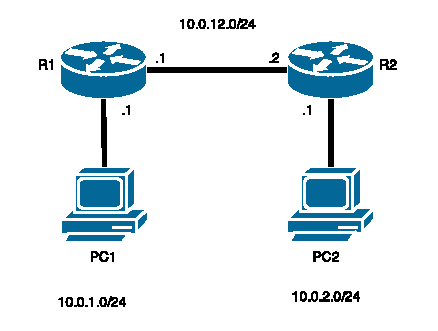
\includegraphics[width=0.6\textwidth]{figures/misc}
            \caption{Physical lab topology.}
            \label{fig:labtop}
        \end{figure}

    \section{Lab experiments}
        \subsection{Setting up a DHCP server }
            \begin{flushright}
                \textbf{[50 points]}\marginnote{\small \textbf{Note:} when done, show your
                work to the lab engineer for grading purposes.}
            \end{flushright}

            \textbf{Important note:} A DHCP server does not have to be in the router. It
            is also recommended to use a dedicated DHCP server depending on the
            load. However, in this lab we will enable the DHCP server that is
            available inside the Cisco router for simplicity only.
            
            DHCP server configuration steps on a Cisco router:
            \begin{enumerate}
                \item \texttt{enable}.
                \item \texttt{config terminal}.
                \item \texttt{service dhcp}.
                \item \texttt{ip dhcp excluded-address <low\_address>
                    <high\_address>}\footnote{This will cause the DHCP server
                        to never lease any IP address in the given interval
                        inclusive. This is used for scenarios where a specific
                        range of IP addresses is statistically assigned to some
                    nodes that might not speak DHCP. For this lab, you may
                    exclude the first $n$ usable IPv4 addresses as long as $n$ is
                    less than 254.}
                \item \texttt{ip dhcp pool <pname>}.
                \item \texttt{network <network\_ip> <subnet\_mask>}.
                \item \texttt{default-router <gateway\_ip\_addr>}.
                \item \texttt{dns-server <dns\_server\_addr>}.
            \end{enumerate}

            Then move to the PCs and perform the following:
            \begin{enumerate}
                \item Most Operating Systems run an implementation of DHCP as a
                    background process. It is possible that, while you were
                    configuring your DHCP server (or reading this text), your
                    PC has obtained its settings. Verify this by executing:
                    \texttt{ifconfig ethX, route -n, cat /etc/resolv.conf} to
                    verify the settings for PC's IP, network mask, default
                    gateway/router, DNS server address respectively.

                \item If the setting is not obtained, you can enforce it as
                    follows: \texttt{dhclient -r} to release the settings (if
                    any), and then \texttt{dhclient} to obtain the settings.
                    This depends on the installed DHCP client.
            \end{enumerate}

            As Wireshark instances were open on the PCs, answer the following
            questions:
            \begin{itemize}
                \item What are the exchanged DHCP message types (e.g.
                    DHCPOFFER) and their direction (e.g. from PC to server)?
                \item What is the purpose of each of the messages?
                \item Which field(s) in which packet(s) contain the IP address
                    that is assigned to your PC?
                \item What are the option codes, lengths and values for
                    network mask, default gateway and DNS server.
            \end{itemize}

            \textbf{Note:} while your clients are configured to use some DNS
            server to resolve names, name resolution will not work as the
            configured DNS server is not configured yet. However, it should
            work once you perform the steps in the next section.

        \subsection{Setting up a DNS server}
            \begin{flushright}
                \textbf{[50 points]}\marginnote{\small \textbf{Note:} when done, show your
                work to the lab engineer for grading purposes.}
            \end{flushright}

            \textbf{Important note:} Using the built-in DNS server of Cisco routers is
            discouraged due to the limited resources on Cisco routers. This lab
            will use the built-in DNS server for demonstration purposes only.
            It is highly recommended to use a more reliable DNS server such as
            Bind9 instead when possible
            
            DNS server configuration steps on a Cisco router:
            \begin{enumerate}
                \item \texttt{enable}.
                \item \texttt{config terminal}.
                \item \texttt{ip dns server}.
                \item \texttt{ip dns primary example.com soa ns.example.com
                    admin.example.com}\footnote{\texttt{example.com} is your
                    point of delegation (i.e. you can authoritatively respond
                    to queries for \texttt{*.example.com} such as
                    \texttt{pc1.example.com}. The address
                    \texttt{ns.example.com} is the primary name server for this
                    domain. \texttt{admin.example.com} is the email address
                    \texttt{admin@example.com} of the administrator of this domain
                    name.}
                \item \texttt{ip host pc1.example.com
                    <ip\_address>}\footnote{This will create a DNS A RR that
                        maps \texttt{pc1.example.com} with
                    \texttt{<ip\_address>}}.
                \item \texttt{ip host pc2.example.com <ip\_address>}.
                \item \texttt{ip host ns.example.com
                    <ip\_address>}\footnote{Use the IP address of the primary
                    DNS server for \texttt{example.com}. Note: to avoid
                    circular dependencies, glue records should be used.}.
            \end{enumerate}
            
            Assuming you're configuration is correct, you should be able to
            use the PCs to \texttt{ping} each other by using their domain names
            instead. E.g. \texttt{ping pc1.example.com} should succeed. If it
            fails, start the debugging process by analysing Wireshark instances
            and observing the output from the DNS server after executing the
            command \texttt{debug domain}.

            Once done, answer the following questions by observing Wireshark
            instances and based on your understanding of the functionality of
            DNS:
            \begin{itemize}
                \item Explain all of the values of the fields in the DNS query.
                    I.e. justify their values.
                \item Explain all of the values of the fields in the DNS reply.
                    I.e. justify their values.
            \end{itemize}


        \subsection{Extra questions (not graded)}
            \begin{itemize}
                \item Describe how can an attacker abuse the DHCP protocol,
                    execute it and then describe a possible solution to the
                    problem.
                \item Describe how can an attacker abuse the DNS protocol
                    (e.g. DNS cache poisoning), execute it, and then describe a
                    possible solution to the problem.
            \end{itemize}

    \appendix
    \section{Relevant protocols}
                \begin{figure}[tbh]
                    \centering
                    \begin{verbatim} 0                   1                   2                   3
 0 1 2 3 4 5 6 7 8 9 0 1 2 3 4 5 6 7 8 9 0 1 2 3 4 5 6 7 8 9 0 1
+-+-+-+-+-+-+-+-+-+-+-+-+-+-+-+-+-+-+-+-+-+-+-+-+-+-+-+-+-+-+-+-+
|Version|  IHL  |Type of Service|          Total Length         |
+-+-+-+-+-+-+-+-+-+-+-+-+-+-+-+-+-+-+-+-+-+-+-+-+-+-+-+-+-+-+-+-+
|         Identification        |Flags|      Fragment Offset    |
+-+-+-+-+-+-+-+-+-+-+-+-+-+-+-+-+-+-+-+-+-+-+-+-+-+-+-+-+-+-+-+-+
|  Time to Live |    Protocol   |         Header Checksum       |
+-+-+-+-+-+-+-+-+-+-+-+-+-+-+-+-+-+-+-+-+-+-+-+-+-+-+-+-+-+-+-+-+
|                       Source Address                          |
+-+-+-+-+-+-+-+-+-+-+-+-+-+-+-+-+-+-+-+-+-+-+-+-+-+-+-+-+-+-+-+-+
|                    Destination Address                        |
+-+-+-+-+-+-+-+-+-+-+-+-+-+-+-+-+-+-+-+-+-+-+-+-+-+-+-+-+-+-+-+-+
|                    Options                    |    Padding    |
+-+-+-+-+-+-+-+-+-+-+-+-+-+-+-+-+-+-+-+-+-+-+-+-+-+-+-+-+-+-+-+-+\end{verbatim}
                    \caption{Internet Protocol (IP) version 4 header format --- Source RFC791.}
                    \label{fig:ipv4}
                \end{figure}

        \begin{figure}[tbh]
                    \begin{center}
                    \begin{verbatim}
               0      7 8     15 16    23 24    31
               +--------+--------+--------+--------+
               | Source Port     | Destination Port|
               +--------+--------+--------+--------+
               |     Length      |    Checksum     |
               +--------+--------+--------+--------+
               |          data octets ...
               +---------------- ...\end{verbatim}
            \end{center}
            \vspace{-15pt}
            \caption{UDP Header Format --- Source: RFC768.}
            \label{fig:udp}
            \vspace{10pt}
        \end{figure}

\end{document}
